Our quantum reinforcement learning architecture consists of three main components:

\subsection{Policy Representation}
The quantum policy $\pi_\theta(a|s)$ is parameterized as:

\begin{equation}
    \pi_\theta(a|s) = |\langle a|U(\theta)|s\rangle|^2
\end{equation}

where $U(\theta)$ is a variational quantum circuit.

\subsection{Learning Algorithm}
We employ a modified Q-learning update rule:

\begin{equation}
    \Delta\theta = \alpha[r + \gamma\max_{a'}Q(s',a') - Q(s,a)]\nabla_\theta Q(s,a)
\end{equation}

\begin{figure}[h]
    \centering
    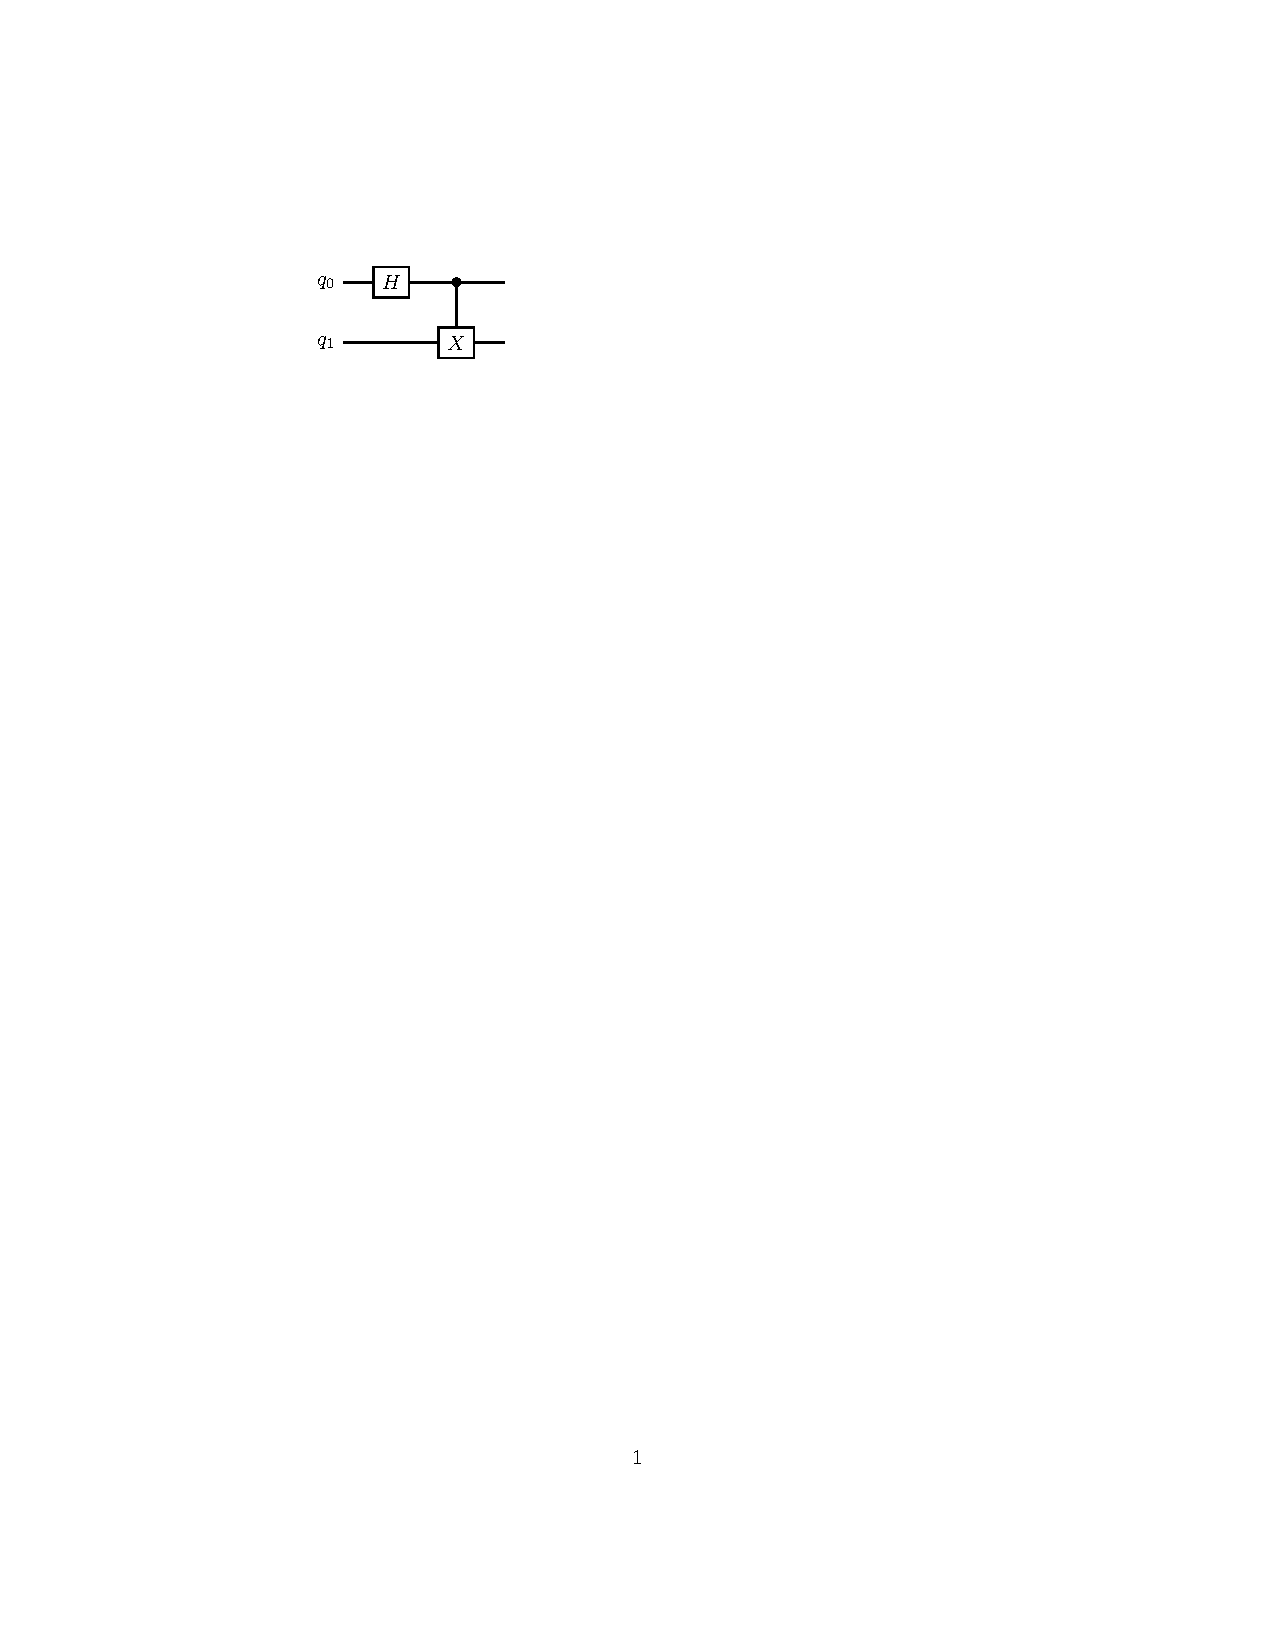
\includegraphics[width=0.7\textwidth]{figures/circuit_diagram}
    \caption{Quantum circuit architecture for policy evaluation}
    \label{fig:circuit}
\end{figure}
